\scanpage{15}
% L1
\[
F\qquad F_U\longrightarrow G_U
\]
\diagram{\begin{tikzcd}[ampersand replacement=\&,column sep=small,row sep=small]
F\arrow[r]\arrow[d] \& i_*(G_U)\\
G\arrow[ur] \&
\end{tikzcd}}
% L2–4
\diagram{\begin{tikzcd}[ampersand replacement=\&,column sep=small,row sep=small]
X\supset U\arrow[dd,"f"'] \& \& \&\\
\& X'\arrow[d,dash]\arrow[r,phantom,"\unsure{\supset|\twoheadrightarrow}"] \& U'\arrow[dl,dash] \& G'\\
Y\arrow[r,dash] \& Y'\arrow[u,bend left=42] \& \substack{\widetilde{x}_1\\[-2pt]\vert\\[-2pt]\widetilde{x}} \& \widetilde{x}'
\end{tikzcd}}
% L3–5 right
\[
A=\varprojlim(A_\alpha=A/\unsure{J_{\alpha+1}|J^{\alpha+1}|I_{\alpha+1}|I^{\alpha+1}|\mathfrak J^{\alpha+1}})\qquad f
\]
\[
\left.\begin{aligned}M&\to{}N\\ M_{\alpha_f}&\xrightarrow{\sim}N_{\alpha_f}\end{aligned}\right|
\Longrightarrow
\left|\begin{aligned}&\forall p\in\operatorname{Spec} A,\\&f\notin p,\\&M_p\simeq N_p\\&(\text{car }\widehat M_p\simeq\widehat N_p)\end{aligned}\right.
\]
% L6 right
\diagram{\begin{tikzcd}[ampersand replacement=\&,row sep=0.3em]
A\arrow[r] \& B\\
\rotatebox{90}{$\subset$} \&\\
\unsure{\mathfrak R|\mathfrak r|\mathfrak A} \& \mathfrak R B
\end{tikzcd}}
\[
(\mathfrak R B\cap A)/\deleted{\mathfrak R}\mathfrak R
\]
% L6–10 left and centre
\[
\begin{aligned}
&\deleted{x_\alpha\in\operatorname{Ass}G_{\unsure{U|X}}}\\
&\deleted{(\Longrightarrow x_\alpha\in\operatorname{Ass}\underline{G_y})}\\
&\deleted{T_\alpha=\overline{\{x_\alpha\}}}
\end{aligned}
\]
\diagram{\begin{tikzcd}[ampersand replacement=\&,row sep=small,column sep=large]
\deleted{x'\in(T_\alpha)_{y'}}\arrow[dd]\arrow[d,dash,bend right=30] \& \text{EGA }\boxed{\mathrm{IV}}\ 12.2.\unsure{.|{}}\\
\text{\deleted{pt maximal}} \& \deleted{\Longrightarrow x'\in\operatorname{Ass}G_{y'}}\arrow[d,Rightarrow]\\
\deleted{y'} \& \deleted{x'\in U_{y'}}
\end{tikzcd}}
% L8–10 right
\[
\deleted{A/\mathfrak R\overset{?}{\hookrightarrow}B/\mathfrak R B}
\qquad A/\mathfrak R_\alpha\hookrightarrow \unsure{B/\alpha'|B\alpha'|B/\alpha|B_\alpha}
\]
\smallskip\hrule\smallskip
% L11–13
\diagram{\begin{tikzcd}[ampersand replacement=\&,row sep=small]
X\arrow[d,"\text{birationnel}"']\\Y
\end{tikzcd}}
\[
\begin{aligned}
&U=\inserted{\text{l'ouvert où } f\ \text{est }\simeq}\unsure{Y|V|\vert},\quad G=O_X,\quad T=X,\quad T_{y'}\ \text{de dim }0\\
&G'\unsure{\simeq|=}O_U,\hspace{9em}T_y\ \text{de dim }1
\end{aligned}
\]
\smallskip\hrule\smallskip
% L14–16 left
\figure{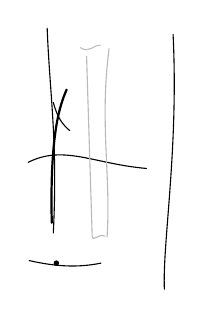
\begin{tikzpicture}[x=0.65cm,y=0.65cm,line cap=round]
\draw (0.6,5.1) .. controls (0.65,3.8) and (0.81,2.9) .. (0.72,1.1);
\draw[thick] (0.98,3.9) .. controls (0.85,3.6) and (0.65,3.05) .. (0.69,1.3);
\draw (0.72,3.65) .. controls (0.8,3.35) and (0.9,3.22) .. (1.04,3.1);
\draw (0.23,2.48) .. controls (0.92,2.83) and (1.51,2.45) .. (2.54,2.36);
\draw[gray!50] (1.25,4.72) .. controls (1.43,4.6) and (1.52,4.79) .. (1.64,4.77);
\draw[gray!55] (1.37,4.55) -- (1.48,1.03) .. controls (1.48,0.92) and (1.6,1.09) .. (1.73,1.04);
\draw[gray!55] (1.81,4.7) .. controls (1.62,3.25) and (1.85,2.2) .. (1.77,1.02);
\draw (0.25,0.56) .. controls (0.78,0.44) and (1.2,0.42) .. (1.65,0.51);
\fill (0.78,0.51) circle (1pt);
\draw (3.06,4.98) .. controls (3.17,2.75) and (2.85,0.88) .. (2.89,0);
\end{tikzpicture}}
% L14–16 centre and right
\diagram{\begin{tikzcd}[ampersand replacement=\&,row sep=small]
x_\alpha\in\operatorname{Ass}G_U\arrow[d,dash]\\ y
\end{tikzcd}}
\[
\begin{aligned}
T_\alpha&=\overline{\{x_\alpha\}}\\
(T_\alpha)_{y'}\cap U&\ \text{est dense ds }(T_\alpha)_{y'}
\end{aligned}
\]
% archive sheet number: 14

